% Source: Code/CommonSenseCarolina/latex/ballot-test.tex
\documentclass[border=0pt]{standalone}
\usepackage{tikz}
\usepackage{xcolor}

\definecolor{BgTop}{HTML}{000000}
\definecolor{BgBottom}{HTML}{1A0A0C}
\definecolor{GarnetDark}{HTML}{4A0006}
\definecolor{Black50}{HTML}{A2A2A2}

\newcommand{\ballot}[4]{% x, y, scale, opacity
  \begin{scope}[shift={(#1,#2)}, scale=#3, opacity=#4]
    \draw[white, line width=0.6pt] (0,0) rectangle (0.4,0.4);
    \draw[white, line width=0.8pt] (0.08,0.18) -- (0.16,0.08) -- (0.34,0.32);
  \end{scope}
}

\begin{document}
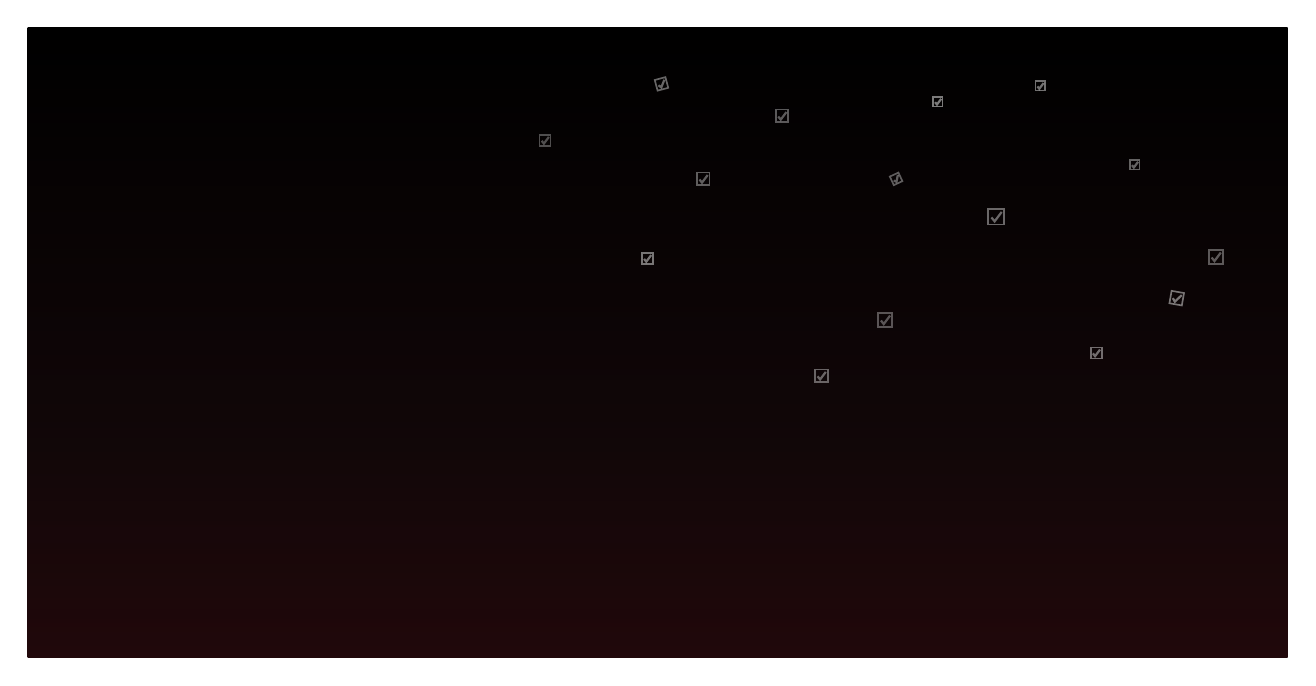
\begin{tikzpicture}

% Dark background
\shade[top color=BgTop, bottom color=BgBottom] (0,0) rectangle (16,8);
\shade[top color=BgBottom, bottom color=GarnetDark, opacity=0.15] (0,0) rectangle (16,2.5);

% Scattered ballots — small and mid sizes, 30-50% opacity
\ballot{9.5}{6.8}{0.4}{0.35}
\ballot{12.2}{5.5}{0.5}{0.40}
\ballot{7.8}{5.0}{0.35}{0.45}
\ballot{14.0}{6.2}{0.3}{0.38}
\ballot{10.8}{4.2}{0.45}{0.32}
\ballot{13.5}{3.8}{0.35}{0.42}
\ballot{8.5}{6.0}{0.4}{0.36}
\ballot{11.5}{7.0}{0.3}{0.48}
\ballot{15.0}{5.0}{0.45}{0.34}
\ballot{6.5}{6.5}{0.35}{0.30}
\ballot{12.8}{7.2}{0.3}{0.44}
\ballot{10.0}{3.5}{0.4}{0.38}

% Some slightly rotated ones
\begin{scope}[rotate around={15:(8.0,7.2)}]
  \ballot{8.0}{7.2}{0.35}{0.40}
\end{scope}
\begin{scope}[rotate around={-10:(14.5,4.5)}]
  \ballot{14.5}{4.5}{0.4}{0.45}
\end{scope}
\begin{scope}[rotate around={25:(11.0,6.0)}]
  \ballot{11.0}{6.0}{0.3}{0.36}
\end{scope}

\end{tikzpicture}
\end{document}
